\documentclass[letterpaper,12pt]{article}
\usepackage{ifthen}
\usepackage{times}
\usepackage{amsmath}
\usepackage{amssymb}
\usepackage{helvet}
\usepackage{courier}
\usepackage{fancyheadings}
\usepackage{hyperref}
\usepackage{comment}
\pagestyle{fancy}
%\usepackage{pmc}
\usepackage{graphicx}
\setlength\textwidth{6.5in}
\setlength\textheight{8.5in}

%%%%%%%%%%%%%%%%%%%%%%%%%%%%%%%%%%%%%%%%%%%%%%%%%%%%%%%%%%%%%%%%%%%%%%%%%%%%%%%%%%
% Special for e-unibus doc commands

\newcommand{\ForLater}{
\begin{center}
{\bf NOT FOR CURRENT VERSION}
\end{center}
}
\newcommand{\TBC}{\framebox{\textbf{TO BE COMPLETED}}}
\newcommand{\DISCUSS}{\Ovalbox {\bf \textcolor{red}{FOR DISCUSSION}}}
\newcommand{\Input}{\framebox{\textsf{in}}}
\newcommand{\Output}{\framebox{\textsf{out}}}
\newcommand{\debug}[1]{\textbf{debug start} #1 \textbf{debug finish}}
\newcommand{\inx}[1]{\emph{#1}}
\newtheorem{notation}{Notation}
\newtheorem{definition}{Definition}
\newtheorem{problem_statement}{Problem Statement}
\newtheorem{invariant}{Invariant}
\newtheorem{assumption}{Assumption}
\newtheorem{resource_string}{Resource String}
\newtheorem{testcase}{Test Case}
\newtheorem{note}{Note}
\newtheorem{specification}{Specification}
\newtheorem{caution}{Caution}
\newtheorem{prereq}{Pre-requisite}
\newtheorem{action}{Action}
\newtheorem{query}{Query}
\newcommand{\beq}{\begin{equation}} %% new, no conflict
\newcommand{\eeq}{\end{equation}} %% new, no conflict
\newcommand{\be}{\begin{enumerate}}
\newcommand{\ee}{\end{enumerate}}
\newcommand{\bi}{\begin{itemize}}
\newcommand{\ei}{\end{itemize}}
\newcommand{\bv}{\begin{verbatim}}
\newcommand{\ev}{\end{verbatim}}
\newcommand{\bd}{\begin{description}}
\newcommand{\ed}{\end{description}}
\newcommand{\bpre}{\begin{prereq}}
\newcommand{\epre}{\end{prereq}}
\newcommand{\bact}{\begin{action}}
\newcommand{\eact}{\end{action}}
\newcommand{\bs}{\begin{specification}}
\newcommand{\es}{\end{specification}}
\newcommand{\btc}{\begin{testcase}}
\newcommand{\etc}{\end{testcase}}
\newcommand{\bc}{\begin{caution}}
\newcommand{\ec}{\end{caution}}
\newcommand{\la}{\leftarrow}
\newcommand{\IpArgs}{\subsection{Input Arguments}}
\newcommand{\PreReqs}{\subsection{Pre-requisities}}
\newcommand{\Actions}{\subsection{Actions}}
\newcommand{\Coverage}{{\bf To test coverage.}}

%%%%%%%%%%%%%%%%%%%%%%%%%%%%%%%%%%%%%%%%%%%%%%%%%%%%%%%%%%%%%%%%%%%%%%%%%%%


\newtheorem{theorem}{Theorem}[section]
\newtheorem{lemma}[theorem]{Lemma}
\newtheorem{proposition}[theorem]{Proposition}
\newtheorem{corollary}[theorem]{Corollary}

\newenvironment{proof}[1][Proof]{\begin{trivlist}
\item[\hskip \labelsep {\bfseries #1}]}{\end{trivlist}}
\newenvironment{intuition}[1][Intuition]{\begin{trivlist}
\item[\hskip \labelsep {\bfseries #1}]}{\end{trivlist}}
%% \newenvironment{definition}[1][Definition]{\begin{trivlist}
%% \item[\hskip \labelsep {\bfseries #1}]}{\end{trivlist}}
\newenvironment{example}[1][Example]{\begin{trivlist}
\item[\hskip \labelsep {\bfseries #1}]}{\end{trivlist}}
\newenvironment{remark}[1][Remark]{\begin{trivlist}
\item[\hskip \labelsep {\bfseries #1}]}{\end{trivlist}}

\newcommand{\qed}{\nobreak \ifvmode \relax \else
      \ifdim\lastskip<1.5em \hskip-\lastskip
      \hskip1.5em plus0em minus0.5em \fi \nobreak
      \vrule height0.75em width0.5em depth0.25em\fi}

%%%%%%%%%%%%%%%%%%%%%%%%%%%%%%%%%%%%%%%%%%%%%%%%%%%%%%%%%%%%%%%%%
% \newcommand{\Alogon}{\mbox{\fontfamily{ptm}\selectfont {\large \selectfont A} \hspace{-1.2ex} {\large \selectfont L} \hspace{-2.3ex} \raisebox{0.45ex}{ {\footnotesize \selectfont O} } \hspace{-1.80ex} {\large \selectfont G} \hspace{-1.80ex} \raisebox{-0.33ex}{ {\large \selectfont O} } \hspace{-1.8ex} {\large \selectfont N}}}



\newcommand{\beq}{\begin{equation}} %% new, no conflict
\newcommand{\eeq}{\end{equation}} %% new, no conflict
\newcommand{\bdm}{\begin{displaymath}} %% new, no conflict
\newcommand{\edm}{\end{displaymath}} %% new, no conflict
% \newcommand{\reals}{{\rm I\! R}} %% new, no conflict
\newcommand{\reals}{\cal{R}} %% new, no conflict
% \newcommand{\mymean}[1]{\mu({#1})}
\newcommand{\bb}[1]{\mathbb{#1}}
\newboolean{longform}
\setboolean{longform}{false}
\newboolean{blogpost}
\setboolean{blogpost}{true}
%% Another option is \usepackage{comment}
%% \includecomment(answer} or excludecomment{answer} % then
%% \begin{answer} ... \end{answer}


%% From https://math.berkeley.edu/~gbergman/misc/hacks/langl_rangl.html
\newcommand{\langl}{\begin{picture}(4.5,7)
\put(1.1,2.5){\rotatebox{60}{\line(1,0){5.5}}}
\put(1.1,2.5){\rotatebox{300}{\line(1,0){5.5}}}
\end{picture}}

\newcommand{\rangl}{\begin{picture}(4.5,7)
\put(.9,2.5){\rotatebox{120}{\line(1,0){5.5}}}
\put(.9,2.5){\rotatebox{240}{\line(1,0){5.5}}}
\end{picture}}

\newcommand{\mymean}[1]{\ensuremath{\langl{#1}\rangl}} %% new, no conflict

\begin{document}
\title{Max.(Minimum Expected Return)}
\author{Ramesh Subramonian, Ranjeet Tate, Michael Shire, Abhi Singh}
\maketitle
\thispagestyle{fancy}
\lhead{}
\chead{}
\rhead{}
\lfoot{}
% \cfoot{{\small NerdWallet Engineering }}
% \rfoot{{\small \thepage}}

\section{Email March 24 2016}
\label{sec:intro}
Sub, this brings back in the idea of some knee we should look for that
you had in the original version of the article.

\subsection{Original end-point}
For a given result set (number of trials and successes for each of
test and control) and for a given comparison metric, currently our
analysis provides our client (prod managment, execs, biz development)
with a plot of comparison metric value vs credibility. For data =
(200, 40, 100, 15).  Figure~\ref{fig:delta_vs_cred}.
\begin{figure}[ht!]
\centering
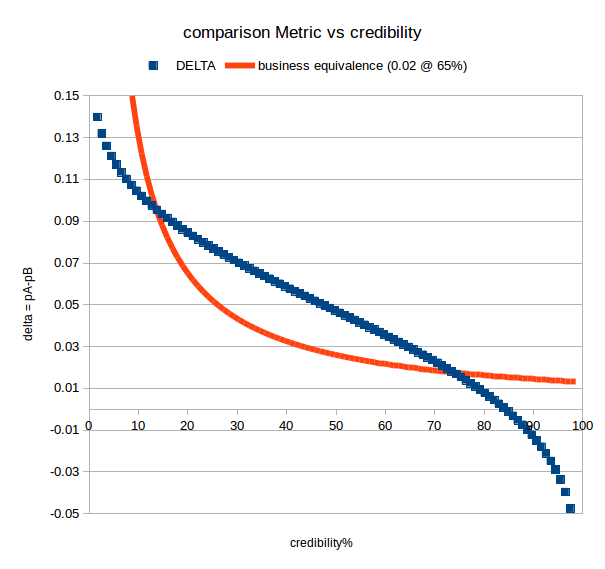
\includegraphics[width=90mm]{delta_vs_cred}
\caption{Delta vs. Credibility \label{fig:delta_vs_cred}}
\end{figure}
We'll discuss the orange line in a minute.

The intended use is that BEFORE even starting the experiment, based on
desired business outcomes, a client can set a threshold for a
particular metric, so if the value of the comparison metric exceeds
that minimum, some business action is triggered. For example a PM
might decide to stick with the simple "difference" metric, and decide
that a difference of 0.02 is enough to trigger a company wide switch
to variant A. So we do our analysis, provide the above plot, and the
PM looks it up and finds a credibility of 70\%.  The first problem is
that we are still allowing the PM a 1-parameter family of fudge
factors. 70\% credibility may seem unacceptably low to them, So they
can change their minds and say oh 0.02 was too ambitious, it only
needs to be better by 0.005, which has a credibility of >80\%, and we
are good to go. I don't want them to have any fudge factor once
they've set their threshold for a metric before starting the test.
More kindly viewed, a PM doesn't want the responsibility of this
choice, and we shouldn't burden our client with choice and the
attendant blame if things were to go wrong. The analysis should yield
a clear no-go/go answer.

\subsection{Expected Minimum Return}
So how do we go about doing this? Assume, as we have been doing so
far, that \(M(x,y)\) has been chosen because it is linear in \$ or profit
or revenue or some tangible business goal. Then we should treat the
value of \(M(x,y)\) as the return and the corresponding credibility(value)
as the probability of that return (this blog
\url{http://jakevdp.github.io/blog/2014/03/11/frequentism-and-bayesianism-a-practical-intro/}
provides sufficient justification for treating Bayesian credibility as
such). Then value * credibility is the expected return.

\subsection{Claim: Expected Minimum Return has a Maximum}\label{sec:exists_max}
In (pA,pB) space, assume any joint PDF.  Then, at large negative value
(curve squished in top left corner), the credibility is 1, so the
expected return is large and negative.  At large positive value,
(curve squished in bottom right), the credibility is 0, so the
expected return is 0.  For any joint PDF, for some finite (even if
small) non-zero value of the comparison metric (curve just bulging
downward from the 45 degree line), say \(\epsilon\), the credibility
is positive (even if small), hence the expected return is positive.
=> From value = 0 to value = \(\epsilon\), the expected return goes
from negative to positive, so by some theorem or the other, the
expected return is zero for value of metric in \(\in
[0,\epsilon]\). Call this point \(\epsilon_0\).  Now, at
\(\epsilon_0\), expected return = 0, and at max value, expected return
= 0. Somewhere in between, we've already shown, at \(\epsilon_0 <
\epsilon < max(value)\), expected return is positive. hence there is
at least one maximum. Since all the functions are finite, we can find
the global finite maximum.

Q.E.D.

The curve looks like 
Figure~\ref{fig:exp_return_vs_delta}.
\begin{figure}[ht!]
\centering
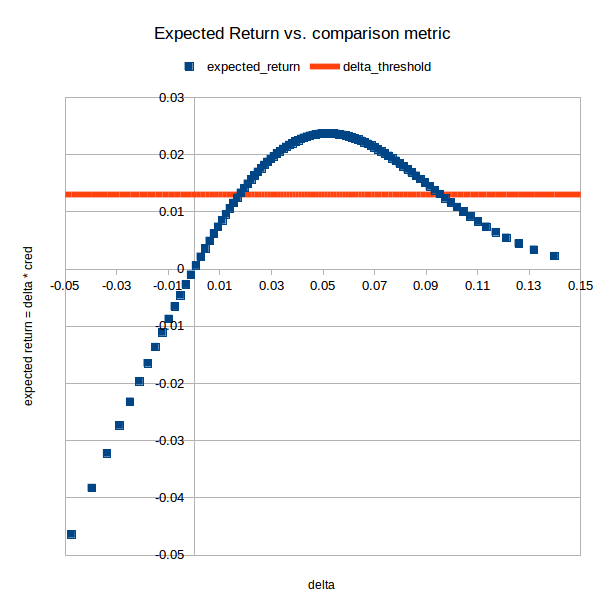
\includegraphics[width=90mm]{expected_return_vs_delta}
\caption{Expected Return vs. Delta \label{fig:exp_return_vs_delta}}
\end{figure}
Just as we proved above.

The question we should ask is whether the max(expected minimum return) > PM's
threshold.  If no, experiment is a failure, if yes, the safe thing to
do is to wait to see how it is trending before making a decision.  My
unproven belief is that this way of doing things, once we are beyond
100 positives, we should be robust.  In the above situation, if the PM
had set 0.02 as the threshold, since the max expected return is
actually > 0.02, we declare it a success.

\section{``Just like life, going in circles.'' -- Old Bulgarian saying}
Okay, that was an absurd rabbit hole. Ramesh asked why this was any
different from simply calculating the mean difference. Thinking about
it: \(p_A = x\) and \(p_B = y\) as in the article.  What I am proposing is
that for every metric \(M\) for comparing A/B, we have a "difference"
parameter \(\delta M(x,y)\) e.g. it is \(\delta M= x-y\) for "delta" and \(\delta M= \ln\left(\frac{o(x)}{o(y)}\right)\) for
odds ratio etc.

I am doing some somewhat funky \(\delta M*credibility(\delta M)\) as an
expected value of \(\delta M\), then maximizing it. Ramesh's question is why
not just take the expectation value of \(\delta M\) to begin with?

Since the difference is a function of \((x,y)\) and we know the joint
probability density, I could just calculate the expected value of the
difference: \(\mymean{\delta M} = \int_x \int_y \delta M(x,y) f_A(x) f_B(y)\)

So instead of the max(expected value(\(\delta M\))), we would compare
the above \(\mymean{\delta M}\). But then we would say, I don't want
to make business decisions based on the mean, I want to be 85\%
confident. So we are back to having to include the credibility as a
parameter.

And how do we calculate the credibility as a function of \(\delta M\)?
We've already done this, in the \(\delta M\) vs credibility curves.

So a lot of thinking, but at least it gets us back to what we were
already doing.

\section{After going around in a circle, back to square 1}
After having rejected the above ``maximum expected value'' approach, I
continued to have some misgivings about the earlier ``metric
vs. credibility'' approach. After all there is a reason that most
people never seem to get it. And think about it, what does a PM do
with a curve like the original curves?

Assume that the \(\delta M \propto \$\), i.e. it is linear in some tangible
business goal.

Since \(\delta M\) is a function on the 2D probability space and we
have the probability distribution on that space, we obtain a
distribution on \(\delta M\). So we can calculate the \(\mymean{\delta
  M}\). What does it {\em not} mean? It does not, due to possible
skewness, mean that \(\delta M >\mymean{\delta M}\) 50\% of the time,
that is a property of the median or the 50th\%\(ile\).

Assume for a moment that the distribution is symmetric. Then we can
say that \(\delta M >\mymean{\delta M}\) 50\% of the time. This gets
us thinking about using a larger, ``safer'' percentile value (which we
refer to as the {\em credibility} in the main article, say \(\delta
M_{95\%}\), which means that \(\delta M >\delta M_{95\%}\) 95\% of the
time. Extending this to other values of credibility leads to the
experimental metric vs. credibility curve, shown in blue in
Figure~\ref{fig:delta_vs_cred}.

What these statements also mean is that our {\em expected minimum
  return} is \(0.5*\mymean{\delta M}\) in the first case and
\(0.95*\delta M_{95\%}\) in the second. {\em This} is the metric we
should be optimizing.

Now let's say you have a business-savvy and statistically
knowledgeable PM, who comes up with a statement like ``If we get
\(\delta M_0 = \$111\) money with \(C_0\% = 90\%\) credibility, that
triggers a business action in favor of A''.  What this means in terms
of Figure~\ref{fig:delta_vs_cred} is that if the experimental metric
vs. credibility curve lies above and to the right of the point
\((\delta M_0, C_0)\) the triggering condition is satisfied.  We will
see that while the simple geometric statement ---that a curve divides
the plane in two disjoint sets, and a point either lies on one side of
the curve or it doesn't--- is unambiguous, the business decision is
{\em not unambiguous}!

How so? Let's consider what really underlies the PM's condition.
Is a less risk-averse
condition that \((\delta M_0, C_0) = (\$125, 80\%)\) really that
different from the first PM's \((\delta M_0, C_0) = (\$111, 90\%)\)?
In fact, they are {\em not} different, they are equivalent from a
business perspective because their expected returns are the same:
\(\$111* 0.90 = \$125* 0.80 = \$100\). There is in fact an equivalence class
of conditions \((\delta M, C)\) which satisfy:
\beq\label{eq:hyperbola}
\delta M*C =\delta M_0*C_0
\eeq
which lead to the same expected returns.  What this means is that if
we were able to guarantee 100\% credibility, the PM would be satisfied
with
\beq
\delta M(Threshold):=\delta M|_{C=100\%}
\eeq
In our case, \(\delta M(Threshold) =\$111*0.90=\$100\), which is the
same value for the expected return. As we can see from the above
equation, this defines a hyperbola in metric-credibility space.

This is the orange curve in Figure~\ref{fig:delta_vs_cred}. One can
see from the general shape of the threshold curve and the experimental
metric vs. credibility curve that they are not part of the same family of
contours and can intersect each other. A further implication of this
is that generically, for every point \((\delta M_0, C_0)\) that lies
below the experimental metric-credibility curve and hence triggers the
business action, there is a \((\delta M_0', C_0')\) ---completely
equivalent from a business perspective--- that lies abve the
metric-credibility curve and does {\em not} trigger the business
action.

What we've shown is that there are choices of \((\delta M_0, C_0)\)
which are equivalent to each other from a business perspective but
which lead to contradictory decisions. So we can't meaningfully ask if
a point \((\delta M_0, C_0)\) lies on one side of a curve or not. What
we should really ask is whether the continuous curve or equivalence
class of points lies entirely on one side of the other curve (which is
not a contour of the same function as the first curve). This is {\em
  not} a geometrically well-defined problem.

What, then, is a way of framing the question so it is a property of
the threshold metric value and not of the specific choice of \(\delta
M_0, C_0\)? We can demand that the {\em entire curve} lie above or
below the metric-crediblity curve. However, because of the shapes of
the two curves, the entire threshold curve can lie on one side of the
metric-credibility curve only if it lies above! Since this corresponds
to the business action {\em not} being triggered, the definitive
answer can only be negative. This is logically fine, recall that most
scientific tests reject the null hypothesis rather than ``accept the
positive''. Re-writing \ref{eq:hyperbola}, the condition becomes
\bdm
\delta M < \frac{\delta M_0 * C_0}{C(\delta M)} \forall \delta M
\edm
Multiplying both sides by the credibility \(C\), and identifying the
right hand side as the metric threshold
\beq
\delta M * C(\delta M) < \delta M(Threshold) \forall \delta M
\eeq
The Left Hand Side is the
minimum expected return, and the above condition is equivalent to:
\bdm
Max(\delta M*C(\delta M)) < \delta M(Threshold)
\edm
This is
shown in Figure~\ref{fig:exp_return_vs_delta}, where the orange line
is the threshold for triggering the business action as established by
the PM. The experimentally obtained blue curve reflects the changes in
the expected minimum return as we increase the value of the metric
while the credibility correspondingly drops. As we've shown in
Section~\ref{sec:exists_max}, this curve has a maximum.

It means that there is no combination of \((\delta M_0', C_0'): \delta
M(Threshold) = \delta M_0'*C_0'\) equivalent to the original \((\delta
M_0, C_0)\) which will lead to triggering the business action: the
entire orange curve lies above the metric-credibility curve. The
result can not be finagled post hoc.

If on the other hand
\bdm
Max(\delta M*C(\delta M)) > \delta M(Threshold)
\edm
then there is some combination of \((\delta M, C): \delta M(Threshold)
= \delta M*C\) which does lead to triggering the business decision:
since the two curves intersect, even if we start on the ``wrong'' side
we can crossover to the ``correct'' side. So we might as well declare
it a win.

This reduces the PM's job to coming up with a single dollar value for
their minimum expected return sufficient to trigger a business
action. It doesn't need to involve any statistical sophistication on
their part.

This is how we should finish with the AB analysis: PM gives a number,
we calculate one number, compare the two and return a win/no-win
response. With all the supporting figures because everybody wants to
see some pictures even if we don't quite understand them.

\section{log(odds factor)}
Similar statements hold for the log(odds factor) if it is directly
proportional to a business financial goal.
Figure~\ref{fig:odds_factor_vs_cred}.
\begin{figure}[ht!]
\centering
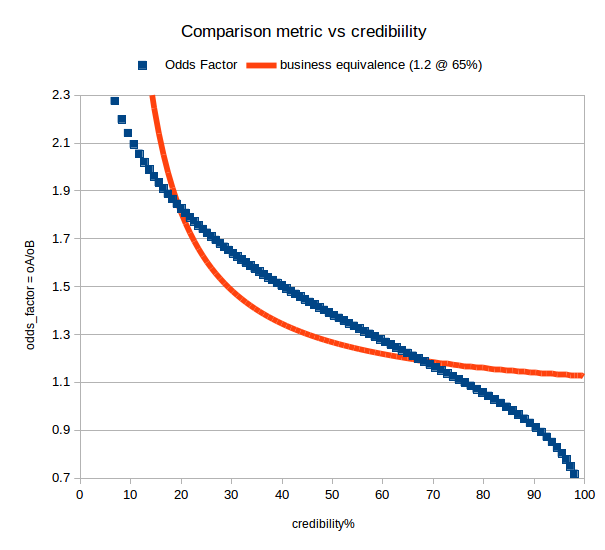
\includegraphics[width=90mm]{odds_factor_vs_cred}
\caption{Odds Factor vs. Credibility \label{fig:odds_factor_vs_cred}}
\end{figure}
and Figure~\ref{fig:exp_return_vs_odds_factor}.
\begin{figure}[ht!]
\centering
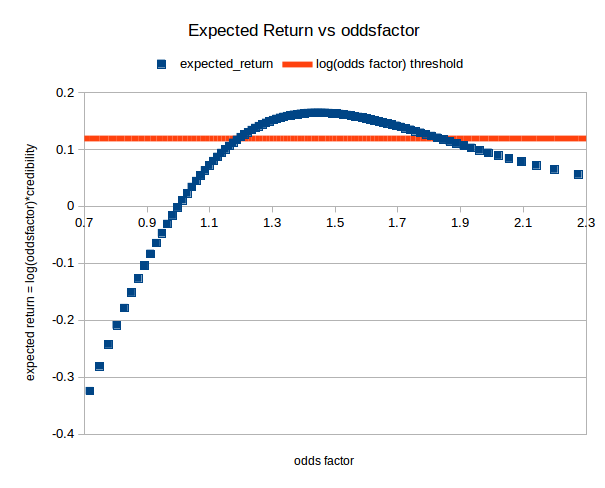
\includegraphics[width=90mm]{expected_returns_vs_odds_factor}
\caption{Expected Return vs. Odds Factor \label{fig:exp_return_vs_odds_factor}}
\end{figure}

\section{Future work}
The interesting thing would be to see how max(minimum expected return) changes
as we scale \(\alpha*(200, 40, 100, 15)\). The more difficult problem would
be to simulate a run, similar to the Optimizely white paper, and see
how max(minimum expected return) evolves as we collect more data.

\end{document}

% SOME BOGUS COMMENT
